%----------------------------------------------------------------------------
\chapter{\FurtherDevelopment}
%----------------------------------------------------------------------------

%----------------------------------------------------------------------------
\section{Üzemeltetési tapasztalatok}
%----------------------------------------------------------------------------

A megvalósított rendszer üzemeltetése a tervezett módon történt. A rendszer
tökéletesen megfelelt a kitett elvárásoknak, és üzemeltetése során nem
tapasztaltunk semmilyen rendellenességet. A teljesítménye és megbízhatósága is megfelelőnek bizonyult, nem 
voltak csomagvesztések a hálózaton, egyetlen egyszer sem kellett a másodlagos redundáns hálózatra
váltani, nem fordultak elő kiugró késések, minden eszköz bőven a beállított buffer méretben belül maradt.
Minden komponens megfelelően végezte a rá bízott feladatot, és a rendszer
stabilan kihagyás nélkül működött a teljes üzemidő alatt. 



% Plusz ötletek:
% mitől  a legjobb a dante, mire képes a szoftver, milyen  limitációk vannak benne, milyen fejlesztési irányelveket fogalmaznál meg, 

% miben könnyíti meg a munkád?

 
 


%----------------------------------------------------------------------------
\section{Továbbfejlesztési lehetőségek}
%----------------------------------------------------------------------------


%----------------------------------------------------------------------------
\subsection{További eszközök integrálása}
%----------------------------------------------------------------------------
A Dante networking keresztrendszer lehetővé teszi a rendszer folyamatos bővítését a
hálózati limitációk megfelelő kezelésével. A rendszer bővítésekor figyelembe kell venni a
még rendelkezésre álló, a sávszélességet és a késleltetést mértékét. Amennyiben
tarjuk magunkat ezekhez a paraméterekhez, a rendszer bővítése nem okozhat problémát,
és megfelelő overhead mellett elméletileg a teljes hálózatot is szaturálhatjuk mindenféle probléma nélkül.
A Martin Audio Wavefront sorozatú hangfalak skálázható felbontása lehetővé teszi, hogy
a rendszer bővítésekor a már meglévő hangrendszerünket több végfokkal hajtva tovább
növeljük a rendszer teljesítőképességét. A korábbiakban már említett felbontás növelés
javítja a rendszer hangminőségét, frekvenciafelbontását és az adott területen való
pontosabb hangeloszlást. Ebből kifolyólag nagy fejlesztés lehet a jövőben a rendszer egy ládás
felbontásra való kibővítése. Ez azt jelenti, hogy az összes Line Array egységet külön-külön
végfok csatornával hajtjuk meg.
További fejlesztés a rendszerben a LineArray hangfalak számának növelése megfelelő számú végfok egységgel,
amely tovább növeli a rendszer teljesítményét és a maximálisan lefedhető területet.
%----------------------------------------------------------------------------
\subsubsection{Shure Axient Digital rendszer} % A jel egyből a Dante hálózaton keresztül érkezik a keverőbe nincs A/D konverzió
%----------------------------------------------------------------------------
A Shure Axient Digital vezeték nélküli mikrofon rendszer a szakma egyik legjobb vezeték nélküli
mikrofon rendszere. A rendszer kiváló hangminőséget, megbízhatóságot és rugalmasságot kínál,
és a Dante hálózaton keresztül könnyen integrálható a már meglévő rendszerbe. A jelenlegi
Shure ULXD vezeték nélküli mikrofon rendszerünk is kiváló minőségű, azonban sajnálatos módon 
csak 48 kHz-es mintavételezési frekvenciával rendelkezik, míg az Axient Digital rendszer 96 kHz-es
mintavételezési frekvenciával rendelkezik. Ezáltal a hangminőség jelentősen javulna a rendszerben,
valamint így integrálhatóvá válna direkt módon a Dante hálózaton keresztül a keverőbe, így
nem lenne szükség a hangot analóg jelekké alakítani, majd vissza. Ezáltal a hangminőség még 
kevésbé romlik.
Mint ez eddigi Dante eszközünket, ezt is a Dante Controller segítségével könnyen konfigurálhatjuk, akár egy fixen
kijelölt csatornatartományban, amelyet a keverőpulton is könnyen beállíthatunk. Így mikor rendezvényre érkezünk,
plug and play módon azonnal használhatjuk a mikrofonokat, nem kell a csatornákat újra össze párosítani.
A Shure Wireless Workbench segítségével a mikrofonokat könnyen monitorozhatjuk, és a rendszer
állapotát is ellenőrizhetjük távolról is. A rendszer bővítése jelentős költségekkel jár, így a
bővítés előtt alaposan mérlegelni kell, hogy valóban szükséges-e.
%----------------------------------------------------------------------------
\begin
    {figure}[H]
    \centering
    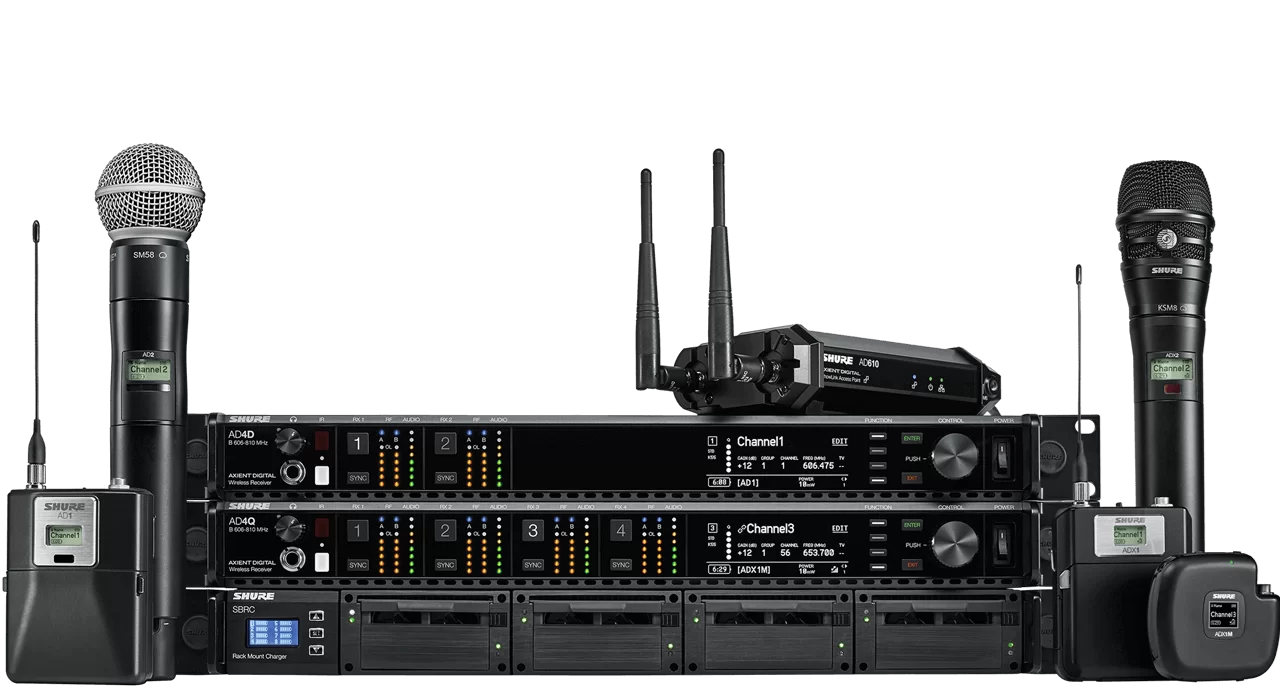
\includegraphics[width=100mm, keepaspectratio]{figures/axient_digital.png}
    \caption{Shure Axient Digital vezeték nélküli mikrofon rendszer}
    \label{fig:shure_axient_digital}
\end{figure}
%----------------------------------------------------------------------------
\subsubsection{TASCAM multitrack recorder} %TASCAM – DA-6400
%----------------------------------------------------------------------------
Egy másik fejlesztési lehetőség a rendszerben egy multitrack recorder beszerzése.
Ez a készülék lehetővé teszi a koncertek soksávos rögzítését, amelyeket később
visszahallgathatunk, vagy akár további feldolgozásra is továbbíthatunk. A TASCAM
DA-6400 egy 64 csatornás, 1U magas rackbe szerelhető multitrack recorder, amely
Dante hálózaton keresztül képes a hangot fogadni és rögzíteni. A felvétel
készítése során a hangot a Dante hálózaton keresztül kapja meg, így nem szükséges
a hangot analóg jelekké alakítani, majd vissza. Ezáltal a hangminőség nem romlik
a felvétel készítése során, és a felvétel készítése is egyszerűbb és gyorsabb lesz.
A felvétel készítése után a felvételt a TASCAM DA-6400-ról egy USB meghajtóra
menthetjük, majd további feldolgozásra továbbíthatjuk. 
%----------------------------------------------------------------------------
\begin
    {figure}[H]
    \centering
    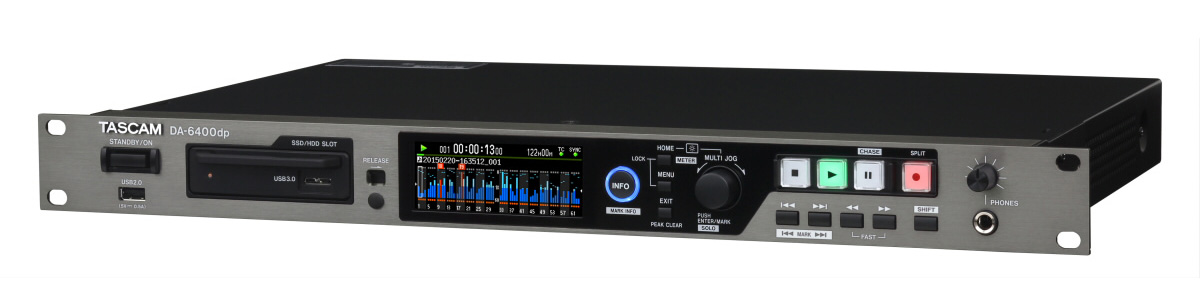
\includegraphics[width=80mm, keepaspectratio]{figures/da_6400.jpg}
    \caption{TASCAM DA-6400 multitrack recorder}
    \label{fig:tascam_da_6400}
\end{figure}
%----------------------------------------------------------------------------

%----------------------------------------------------------------------------
\subsubsection{Allen \& Heath ME Personal Mixing System} % Előadóknak egyéni keverési lehetőség
%----------------------------------------------------------------------------
% ME-U + M-DANTE kártya + ME-500


%----------------------------------------------------------------------------
\subsubsection{Martin Audio WPL LineArray rendszer} % Nagyobb rendezvényekre
%----------------------------------------------------------------------------
Amennyiben egy sokkal nagyobb rendezvényről van szó, és a jelenlegi rendszerünk már nem
tudná lefedni a területet, akkor a rendszer bővítése mellett egy nagyobb szériás LineArray
rendszer beszerzése is szükséges lehet. A Martin Audio WPL sorozatú ládái a jelenleg
elérhető legnagyobb terméke a Wavefront Precision sorozatban. 
Ebben az esetben a fő rendszert a WPL képviselné és WPC lenne az in-out fill rendszer.
A WPM szériás ládák pedig delayként szolgálnának a terület hátsó részén.
Viszont az említett teljes rendszerbővítésnek jelentős költségei vannak, így a rendszer
bővítése előtt alaposan mérlegelni kell, megtérül-e a befektetés hosszabb távon.
%----------------------------------------------------------------------------
\begin
    {figure}[H]
    \centering
    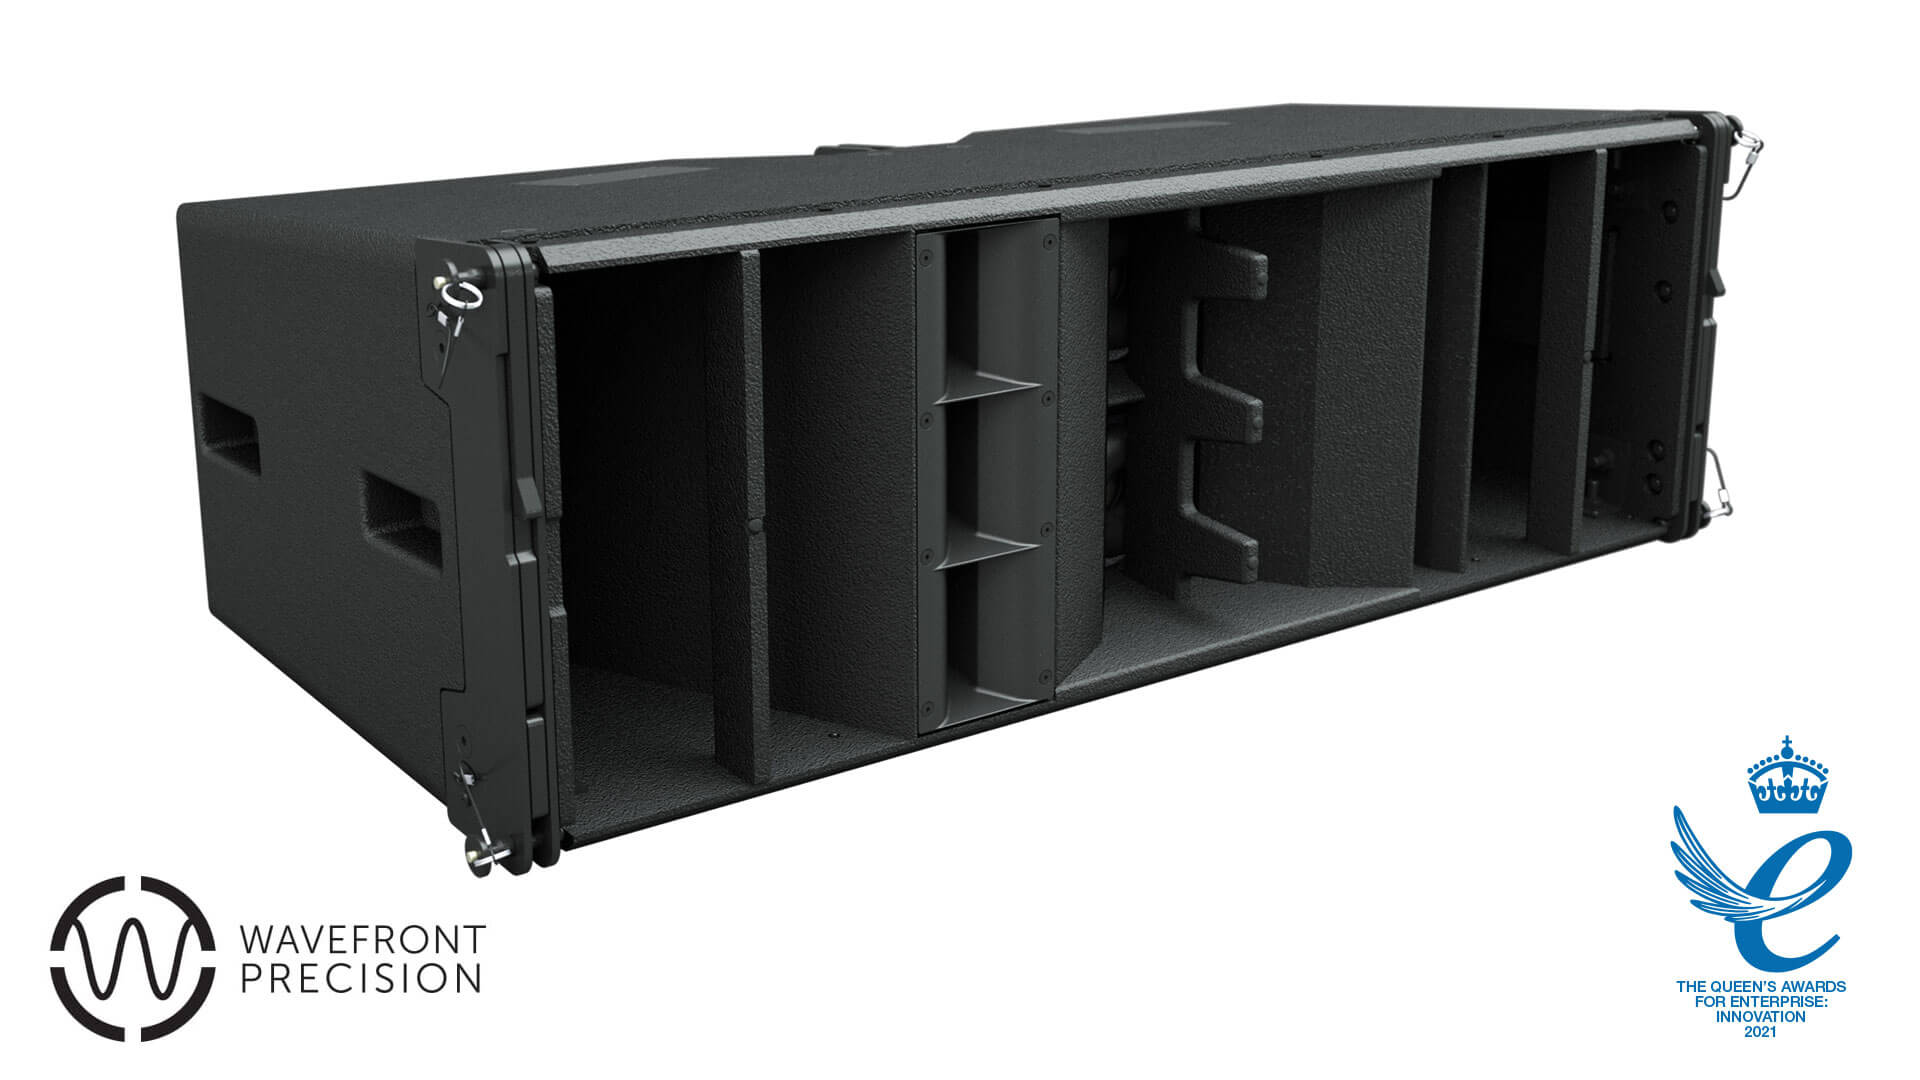
\includegraphics[width=80mm, keepaspectratio]{figures/wpl_front_view.jpg}
    \caption{Martin Audio WPL LineArray modul}
    \label{fig:martin_audio_wpl}
\end{figure}
%----------------------------------------------------------------------------
%----------------------------------------------------------------------------
\subsection{Bővítés nagyobb interfészre és keverőpultra}
%----------------------------------------------------------------------------
Tegyük fel, hogy egy szimfonikus zenekar koncertjét szeretnénk hangosítani, ahol a zenekar
tagjainak száma meghaladja a 64 főt és mindenki dedikált mikrofonnal rendelkezik. Ebben az
esetben a 64x64-es Dante interfész már nem elegendő, mivel a zenekar tagjainak száma
meghaladja a csatornaszámot. Ebben az esetben a rendszer bővítésére van szükség.
Így az Allen \& Heath SQ sorozatú keverőpultjai már nem elegendőek, mivel ezekbe a keverőkbe ez az interfész a maximális.
Ebben az esetben egy nagyobb csatornaszámú keverőpultot kell választanunk, amelyek közül a
az Avantis és a dLive sorozatú keverők jöhetnek szóba. Ezek a keverők már kaphatóak
128x128-as Dante interfésszel is, így megnövelve a csatornaszámot. Azonban ezek a keverők
jelentősen magasabb árkategóriába tartoznak, mint az SQ sorozatú keverők, így a bővítés
költsége is nagyobb lesz. A keverőpultok fejlesztése mellett szükséges további
stageboxokat is beszerezni az igényelt csatornaszám eléréséhez.
%----------------------------------------------------------------------------
\begin
    {figure}[H]
    \centering
    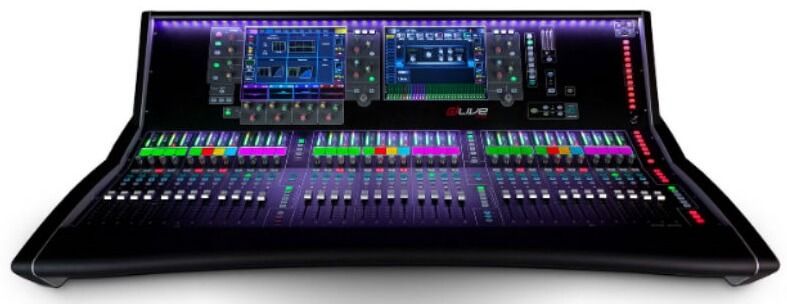
\includegraphics[width=80mm, keepaspectratio]{figures/dlive-s7000.jpg}
    \caption{Allen \& Heath dLive S7000 keverőpult}
    \label{fig:dLive_S7000}
\end{figure}
%----------------------------------------------------------------------------